\newpage
{\bfseries МРНТИ 61.51.29}
\hfill {\bfseries \href{https://doi.org/10.58805/kazutb.v.2.23-484}{https://doi.org/10.58805/kazutb.v.2.23-484}}

\sectionwithauthors{Popov A.Y.}{PRODUCTION OF SYNTHETIC HYDROCARBONS USING COBALT CATALYSTS BASED ON ZSM-5 ZEOLITE}

\begin{center}
{\bfseries A.Y. Popov}

Omsk State Technical University, Omsk, Russian Federation

\envelope Corresponding author: popov\_a\_u@list.ru
\end{center}

In this work, cobalt catalysts based on zeolite ZSM˗5 were prepared by
the triple impregnation method and chemically analyzed. Zirconium
dioxide was used as a promoter (3 wt. \%). Chemical analysis of the
elemental composition and structure of the obtained catalysts was
carried out using scanning electron microscopy. It is shown that the
elemental composition of the catalysts with satisfactory accuracy
corresponds to their given composition. Experiments for catalytic tests
of the prepared catalysts were carried out on a laboratory
Fischer-Tropsch synthesis unit and synthetic hydrocarbons were obtained.
Comparative characterization of activity of the obtained catalysts with
cobalt content of 10 \% and 20 \% has been carried out, dependence of
carbon monoxide conversion and selectivity with respect to formation of
gas hydrocarbons and yield of liquid products on temperature has been
studied.

{\bfseries Keywords:} synthesis gas, cobalt catalysts, promoter,
Fischer-Tropsch synthesis, conversion, selectivity, hydrocarbons

\begin{center}
{\large\bfseries ZSM-5 ЦЕОЛИТ НЕГІЗІНДЕГІ КОБАЛЬТ КАТАЛИЗАТОРЛАРЫН ҚОЛДАНУ АРҚЫЛЫ СИНТЕТИКАЛЫҚ КӨМІРСУТЕКТЕРДІ АЛУ}

{\bfseries А.Ю. Попов}

Омск мемлекеттік техникалық университеті, Омск, Ресей Федерациясы,

e-mail: popov\_a\_u@list.ru
\end{center}

Жұмыста үш есе сіңдіру әдісімен ZSM5 цеолитіне негізделген кобальт
катализаторлары дайындалды және олардың химиялық талдауы жүргізілді.
Промотор ретінде цирконий диоксиді қолданылды (3 мас. \%). Растрлық
электронды микроскопияны қолдана отырып, алынған катализаторлардың
элементтік құрамы мен құрылымына химиялық талдау жасалды.
Катализаторлардың элементтік құрамы олардың берілген құрамына
қанағаттанарлық дәлдікпен сәйкес келетіні көрсетілген. Фишер-Тропш
синтезінің зертханалық қондырғысында дайындалған катализаторларды
каталитикалық сынау үшін эксперименттер жүргізілді және синтетикалық
көмірсутектер алынды. Кобальт мөлшері 10\% және 20 болатын алынған
катализаторлардың белсенділігіне салыстырмалы сипаттама жасалды \%, газ
көмірсутектерінің түзілуіне және сұйық өнімдердің шығымына қатысты
көміртегі тотығының конверсиясы мен селективтілігінің температураға
тәуелділігі зерттелді.

{\bfseries Түйін сөздер:} синтез-газ, кобальт катализаторлары, промотор,
Фишер-Тропш синтезі, конверсия, селективтілік, көмірсутектер.

\begin{center}
{\large\bfseries ПОЛУЧЕНИЕ СИНТЕТИЧЕСКИХ УГЛЕВОДОРОДОВ С ПРИМЕНЕНИЕМ КОБАЛЬТОВЫХ
КАТАЛИЗАТОРОВ НА ОСНОВЕ ЦЕОЛИТА ZSM-5}

{\bfseries А.Ю. Попов}

Омский государственный технический университет, Омск,

Российская Федерация,

e-mail: popov\_a\_u@list.ru
\end{center}

В работе приготовлены кобальтовые катализаторы на основе цеолита ZSM˗5
методом тройной пропитки и проведен их химический анализ. В качестве
промотора использовали диоксид циркония (3 мас. \%). С применением
растровой электронной микроскопии проведен химический анализ элементного
состава и структуры полученных катализаторов. Показано, что элементный
состав катализаторов с удовлетворительной точностью соответствует их
заданному составу. Проведены эксперименты для каталитических испытаний
приготовленных катализаторов на лабораторной установке синтеза
Фишера-Тропша и получены синтетические углеводороды. Проведена
сравнительная характеристика активности полученных катализаторов с
содержанием кобальта 10 \% и 20 \%, изучена зависимость конверсии оксида
углерода и селективность в отношении образования газовых углеводородов и
выхода жидких продуктов от температуры.

{\bfseries Ключевые слова:} синтез-газ, кобальтовые катализаторы, промотор,
синтез Фишера-Тропша, конверсия, селективность, углеводороды.

\begin{multicols}{2}
{\bfseries Introduction.} One of the typical heterogeneous catalytic
processes is the Fischer-Tropsch synthesis, which serves as the basis
for technologies for the production of hydrocarbons from various organic
raw materials and is of great importance for the use of alternative
types of motor fuels and environmental protection {[}1, 2{]}.

Fischer-Tropsch synthesis is a key stage in the technology for producing
synthetic oil and high-quality fuel components from carbon-containing
raw materials. In recent years, the technology has received increasing
attention as an alternative to tapping dwindling oil reserves. The
solution of environmental problems, for example, such as the utilization
of associated gas, adds relevance {[}3-5{]}.

In recent decades, a large number of studies have been carried out in
the field of developing new catalysts for FT synthesis {[}6-9{]}. At the
same time, individual oxides and mixed oxide systems that are prone to
the formation of solid solutions or spinel structures are usually used
as supports for Fischer-Tropsch synthesis catalysts (especially cobalt
ones) {[}10{]}. Typical carriers of Co-catalysts are: silica gel,
kieselguhr, oxides of aluminum, silicon, titanium, magnesium and
zirconium, amorphous aluminosilicates, zeolites. The nature of the
carrier and its physicochemical characteristics can have a strong impact
on the activity and selectivity of contacts. The carrier can also enter
into a chemical interaction with the metal; the carrier participates in
the formation of new compounds or new phases. Strong interaction between
a metal and a carrier can occur through the charge transfer mechanism
with the appearance of a partial positive charge on the metal {[}11{]}.
Basically, with increasing carrier acidity, the yield of liquid and
solid hydrocarbons increases {[}12{]}.

Promising catalysts for the Fischer-Tropsch synthesis are cobalt
catalysts, in the presence of which oxygen-containing and aromatic
hydrocarbons are practically not formed {[}13,14{]}. Cobalt catalysts
have become widespread due to their high activity, durability, and high
selectivity to saturated linear paraffins. In addition, Co-catalysts are
considered the optimal choice for the production of long-chain
hydrocarbons (C\textsubscript{5+}), at moderate temperatures and
pressures {[}15,16{]}.

The objectives of this work are: obtaining synthetic hydrocarbons from
carbon monoxide and hydrogen on cobalt catalysts based on ZSM-5 zeolite
(promoted with zirconium dioxide); study of the temperature dependence
of carbon monoxide conversion and the yield of hydrocarbon products;
study of the influence of cobalt content on the main parameters of
Fischer-Tropsch synthesis.

{\bfseries Materials and methods.} Granular zeolite ZSM-5 was used as a
cobalt catalyst carrier, and zirconium dioxide ZrO\textsubscript{2}
served as a promoter, which was used to increase the activity of the
catalyst and selectivity in the formation of synthetic hydrocarbons. To
prepare cobalt catalysts, the following reagents were used: cobalt
nitrate hexahydrate
(Co(NO\textsubscript{3})\textsubscript{2}·6H\textsubscript{2}O) and
zirconium nitrate hexahydrate
(ZrO(NO\textsubscript{3})\textsubscript{2}·2H\textsubscript{2}O).

Cobalt catalysts were prepared by the triple impregnation method.
Previously, the carrier was pierced in a muffle furnace at a temperature
of 450 \textsuperscript{0}C for 5 hours to remove foreign substances
(including especially carbon).

Cobalt catalysts of the following compositions were prepared: 10\%
Co/3\% ZrO\textsubscript{2}/87\%zeolite ZSM-5 and 20\% Co/3\%
ZrO\textsubscript{2}/77\%zeolite ZSM-5. Previously, the cobalt catalysts
were pre-activated (reduced) in a stream of hydrogen at atmospheric
pressure and a temperature of 350 \textsuperscript{0}C with a volumetric
flow rate of synthesis gas of 1000 h\textsuperscript{-1} for 1 hour.

Catalytic tests on these catalysts were carried out in a laboratory
Fischer-Tropsch synthesis unit at a pressure of 15 atm. in the
temperature range 180-220 \textsuperscript{0}C. Synthesis gas with a
molar ratio of H\textsubscript{2}/CO = 2/1 was supplied at a
successively increased temperature in increments of 10
\textsuperscript{0}C. The duration of the Fischer-Tropsch synthesis
under isothermal conditions at a volumetric flow rate of synthesis gas
of 500 h\textsuperscript{-1} was about 12 hours.

The study of the elemental composition and structural features of the
catalysts was carried out using a Hitachi TM3030 scanning electron
microscope with a Bruker XFlash MIN SVE microanalysis system at an
accelerating voltage of 15 kV.

{\bfseries Results and Discussion.} Figure 1, using the scanning electron
microscopy (SEM) method, shows the results of an analysis of the
composition and structural features of the prepared cobalt catalyst
20\%Co/3\%ZrO\textsubscript{2}/77\%zeolite ZSM-5, which shows the atomic
and weight fraction of the element in the cobalt catalyst based on
zeolite This EDS spectrum contains information about the characteristic
peaks of the sample and the chemical elemental composition of the cobalt
catalyst with the composition 20\%Co/3\%ZrO\textsubscript{2}/77\%zeolite
ZSM-5.

Analysis of SEM images showed that the resulting catalyst with the
composition 20\% Co/3\%ZrO2/77\%zeolite ZSM-5 had pore sizes from 0.3 to
0.7 μm (Figure 2, A). As can be seen from Figure 2 (B), the particle
size of the cobalt catalyst is approximately ≈13-16 μm.
\end{multicols}

\begin{figure}[H]
	\centering
	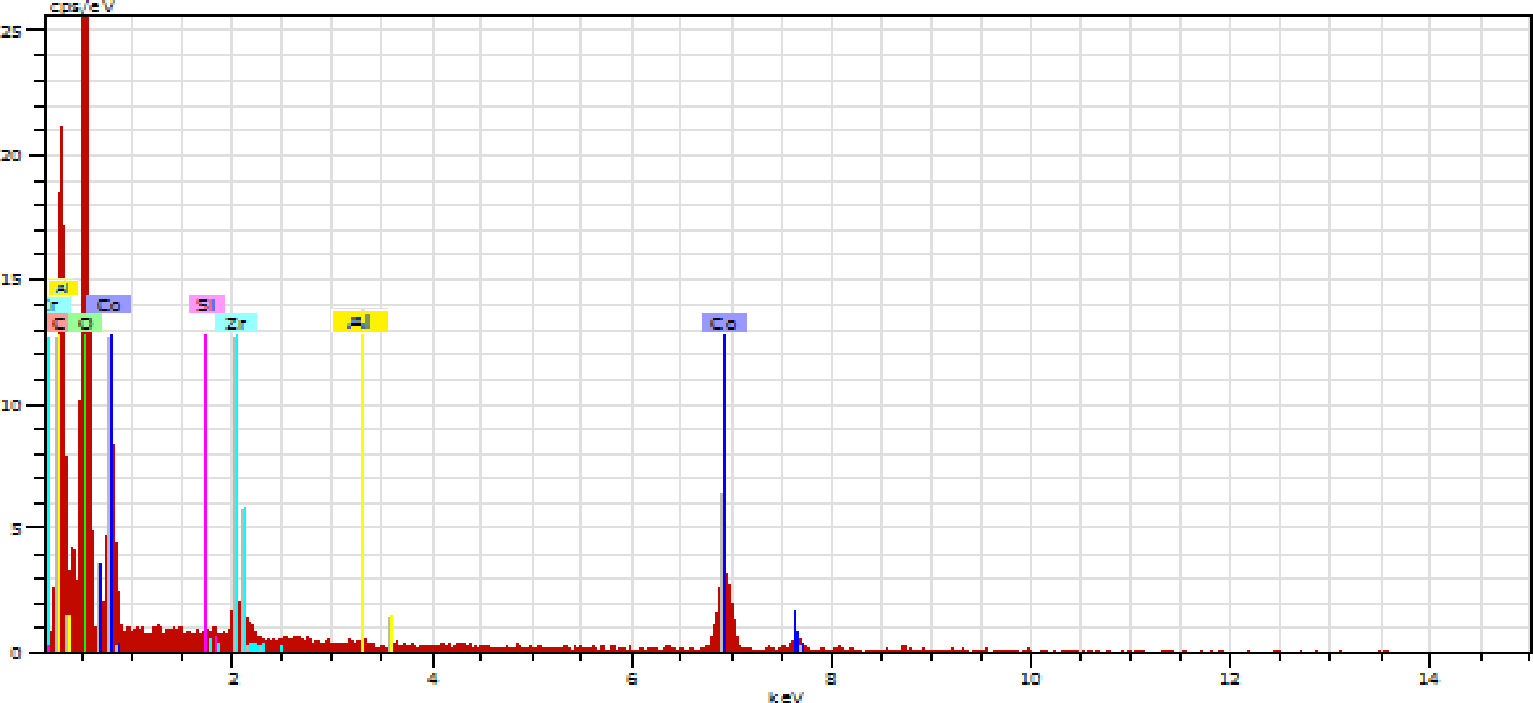
\includegraphics[width=\textwidth]{assets/1076}
  \caption*{Figure 1 -- EDS spectrum of a cobalt catalyst based on zeolite (20\%Co/3\%ZrO2/77\%zeolite ZSM-5)}
\end{figure}

Spectrum: Point

Element AN Series Net unn. C norm. C Atom. C Error

{[}wt.\%{]} {[}wt.\%{]} {[}at.\%{]} {[}\%{]}
\vspace{1em}
\hrule
\vspace{1em}

Oxygen 8 K--series 4029 64.34 48.88 49.39 8.5

Carbon 6 K--series 2380 45.13 34.29 46.15 6.4

Cobalt 27 K--series 1002 19.21 14.59 4.00 0.6

Zirconium 40 L--series 448 2.73 2.07 0.37 0.1

Silicon 14 K--series 36 0.13 0.10 0.06 0.0

Aluminium 19 K--series 17 0.08 0.06 0.03 0.0

\vspace{1em}
\hrule
\vspace{1em}

\hfill Total: 131.62 100.00 100.00

\begin{figure}[H]
    \centering
    \begin{subfigure}[b]{0.45\textwidth}
        \centering
        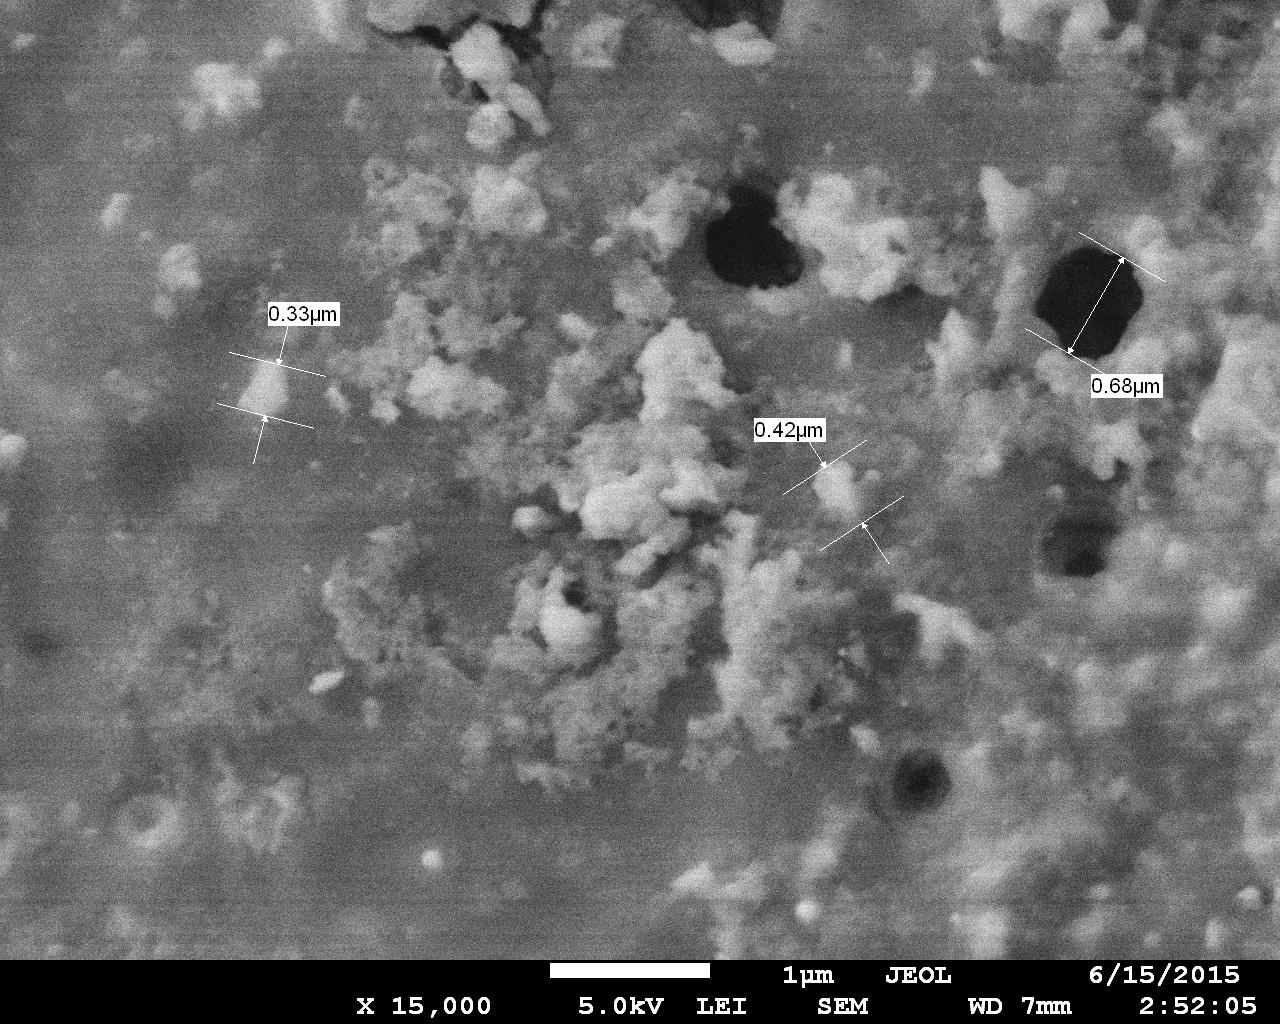
\includegraphics[width=\textwidth]{assets/1077}
        \caption*{A}
    \end{subfigure}
    \hfill
    \begin{subfigure}[b]{0.45\textwidth}
        \centering
        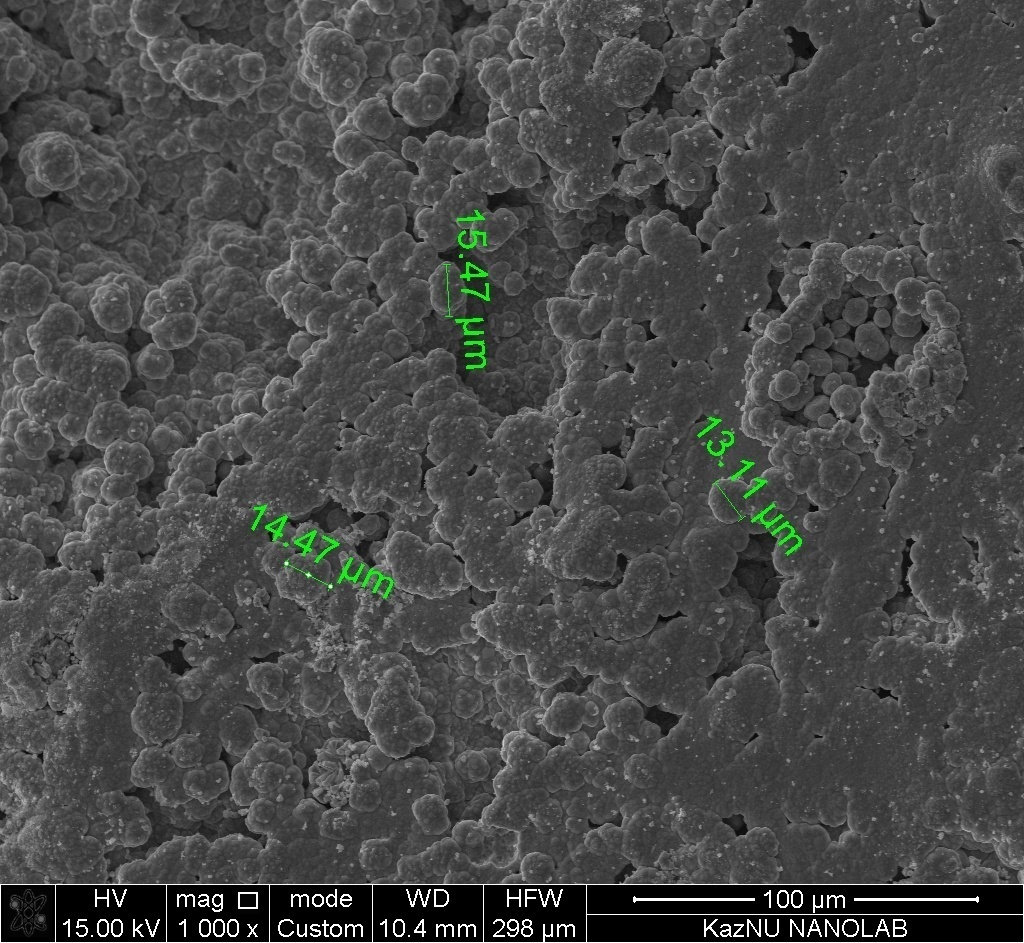
\includegraphics[width=\textwidth]{assets/1078}
        \caption*{B}
    \end{subfigure}
    \caption*{Figure 2 -- SEM images of a cobalt catalyst based on zeolite\\ 20\% Co/3\% ZrO2/77\%zeolite ZSM-5}
\end{figure}

\begin{multicols}{2}
A more detailed study revealed that large fractions of particles of the
catalyst under study were coated with a layer of cobalt and zirconium in
a percentage ratio of 7:1.

Analysis of the data obtained showed that the elemental composition of
the prepared catalysts, determined using scanning electron microscopy,
corresponds with their specified composition with satisfactory accuracy.

Figures 3 and 4 show chromatograms, respectively, of gaseous (at a
temperature of\\
210\textsuperscript{0} C) and liquid products (at a temperature of 200
\textsuperscript{0}C) of synthesis on the catalyst 20\% Co/3\%
ZrO\textsubscript{2}/77\% zeolite ZSM-5 (at their highest
concentrations).
\end{multicols}

\begin{figure}[H]
	\centering
	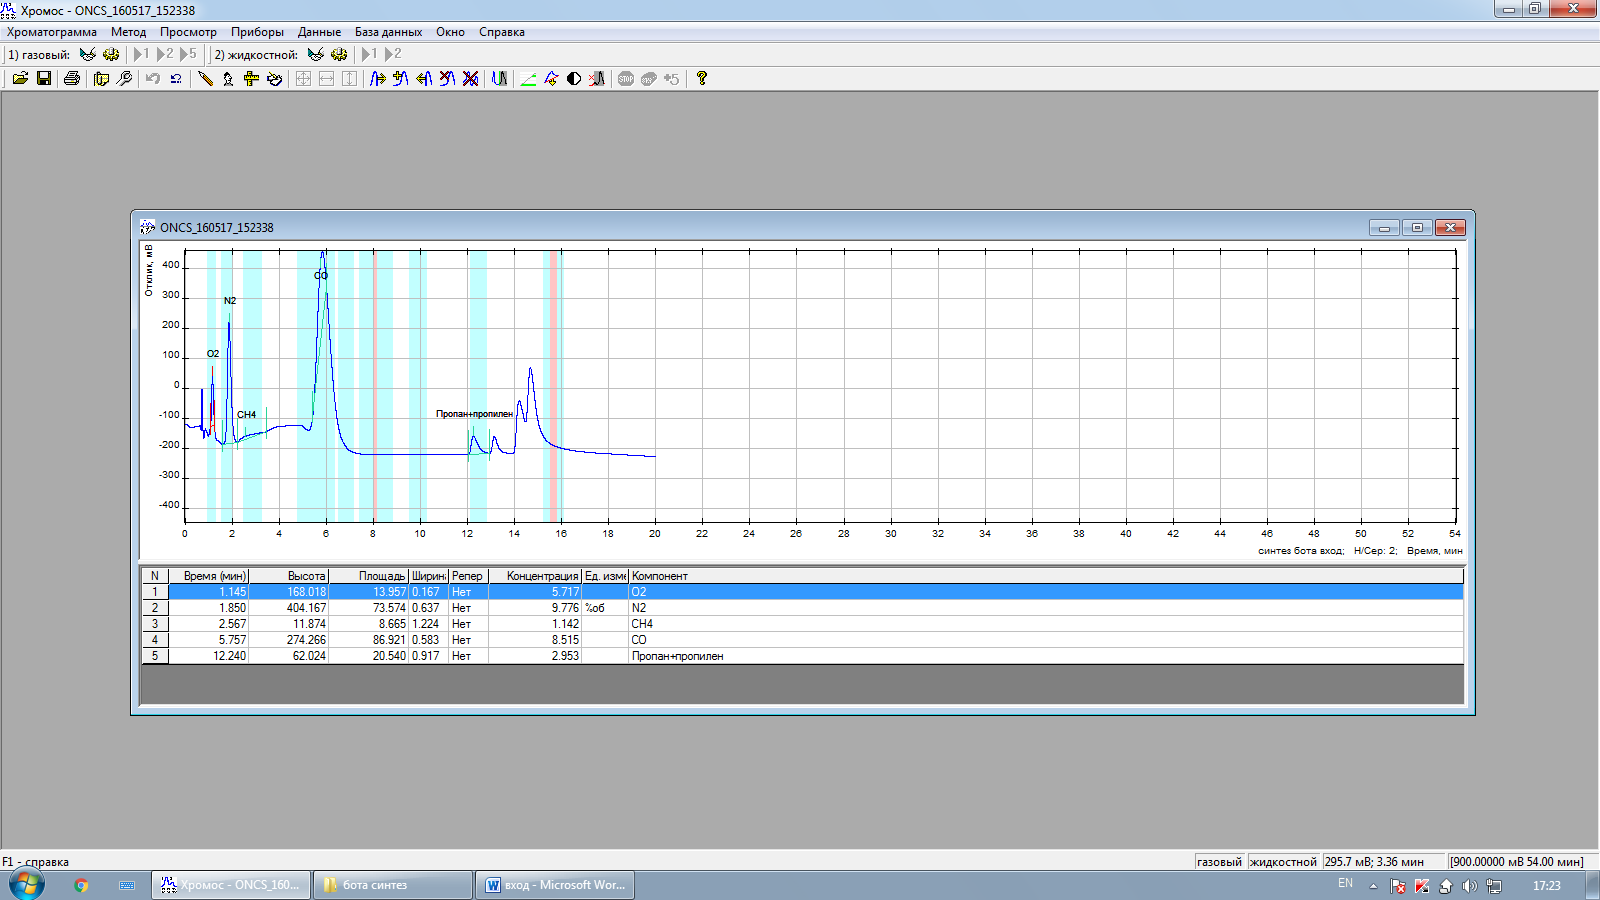
\includegraphics[width=0.8\textwidth]{assets/1079}
	\caption*{Figure 3 -- Chromatogram of gaseous synthesis products on the catalyst 20\%Co/3\%ZrO\textsubscript{2}/77\%zeolite ZSM-5 at a temperature of 210 \textsuperscript{0}C}
\end{figure}

\begin{figure}[H]
	\centering
	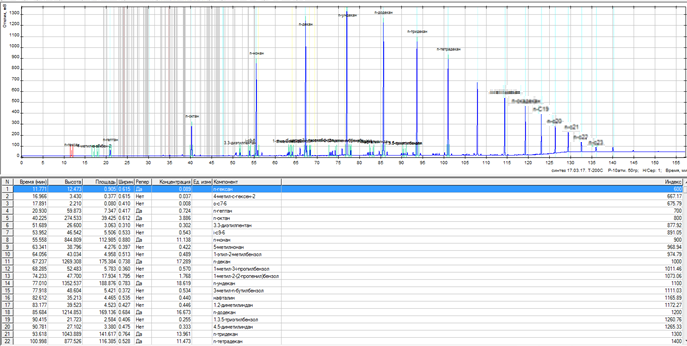
\includegraphics[width=0.8\textwidth]{assets/1080}
	\caption*{Figure 4 -- Chromatogram of liquid synthesis products on the catalyst 20\%Co/3\%ZrO\textsubscript{2}/77\%zeolite ZSM-5 at a temperature of 200 \textsuperscript{0}C}
\end{figure}

\begin{multicols}{2}
The results of the studies on the production of synthetic hydrocarbons
are presented in Tables 1-3, which show the corresponding dependences of
the conversion of carbon monoxide and the concentration of
C\textsubscript{1}-C\textsubscript{4} products on the synthesis
temperature on catalysts 10\% Co/3\% ZrO\textsubscript{2}/87\%zeolite
ZSM-5 and 20\% Co/3\%ZrO\textsubscript{2}/77\%zeolite ZSM-5 with cobalt
content of 10 and 20 wt.\%.

In Table 3, the yield of liquid C\textsubscript{5+} products
(g/m\textsuperscript{3}) of the FT synthesis process on the catalysts
under study was obtained throughout the entire duration of the
synthesis.
\end{multicols}

\begin{table}[H]
\caption*{Table 1 - Main parameters of the Fischer-Tropsch synthesis on the catalyst 10\%Co/3\% ZrO\textsubscript{2}/87\%zeolite ZSM-5}
\centering
\begin{tabular}{|l|l|l|}
\hline
Температура, \tsp{o}С & Конверсия СО, \% & С\tsb{1} – С\tsb{4}\% \\ \hline
180 & \textit{21,5} & \textit{3,7} \\ \hline
185 & \textit{27,4} & \textit{7,3} \\ \hline
190 & \textit{31,6} & \textit{9,4} \\ \hline
195 & \textit{35,5} & \textit{15,2} \\ \hline
200 & \textit{42,1} & \textit{19,3} \\ \hline
205 & \textit{48,2} & \textit{22,1} \\ \hline
210 & \textit{58,8} & \textit{19,8} \\ \hline
220 & \textit{62,7} & \textit{17,3} \\ \hline
\end{tabular}
\end{table}

\begin{table}[H]
\caption*{Table 2 - Main parameters of the Fischer-Tropsch synthesis on the catalyst 20\%Co/3\% ZrO\textsubscript{2}/77\%zeolite ZSM-5}
\centering
\begin{tabular}{|l|l|l|}
\hline
Температура, 0С & Конверсия СО, \% & С1 – С4\% \\ \hline
180 & \textit{28,7} & \textit{4,9} \\ \hline
185 & \textit{31,6} & \textit{8,1} \\ \hline
190 & \textit{37,4} & \textit{11,8} \\ \hline
195 & \textit{45,9} & \textit{18,7} \\ \hline
200 & \textit{54,8} & \textit{20,6} \\ \hline
205 & \textit{67,1} & \textit{26,9} \\ \hline
210 & \textit{70,2} & \textit{28,4} \\ \hline
220 & \textit{79,2} & \textit{25,3} \\ \hline
\end{tabular}
\end{table}

\begin{table}[H]
\caption*{Table 3 - Yield of liquid products of the Fischer-Tropsch synthesis process on the catalysts under study}
\centering
\begin{tabular}{|l|l|l|}
\hline
Catalysts & Temperature, \tsp{o}C & Yield C\tsb{5+}, g/m\tsp{3} \\ \hline
\textit{10\%Co/3\%ZrO2/87\% zeolite ZSM-5} & 210 & 75 \\ \hline
\textit{20\%Co/3\%ZrO2/77\% zeolite ZSM-5} & 200 & 89 \\ \hline
\end{tabular}
\end{table}

\begin{multicols}{2}
Analysis of the data obtained showed that during the synthesis on the
catalyst\\
10\% Co/3\% ZrO\textsubscript{2}/87\%zeolite ZSM-5 with an increase in
temperature from 180 \textsuperscript{0}C to 220 \textsuperscript{0}C,
the main indicators of the process significantly increase: conversion of
carbon monoxide (21.5-62.7 \%), selectivity for the formation of
C\textsubscript{1}-C\textsubscript{4} hydrocarbons (3.7-22.1\%) and the
yield of C\textsubscript{5+} liquid products. At the same time, the
optimal temperatures at which the largest amount of hydrocarbons are
formed are 205 \textsuperscript{0}C and 210 \textsuperscript{0}C for gas
and liquid products, respectively.

Using the catalyst 20\%Co/3\%ZrO\textsubscript{2}/77\%zeolite ZSM-5,
with increasing temperature (180-220\textsuperscript{0}C), the
conversion of carbon monoxide (28.7-79.2\%) and the selectivity of
C\textsubscript{1}-C\textsubscript{4} hydrocarbons (4.9-28.4) and the
yield of liquid C\textsubscript{5+} products. At temperatures of 210
\textsuperscript{0}C and\\
200\textsuperscript{0}C, the largest amounts of gas and liquid
hydrocarbons are formed, respectively.

The obtained experimental results showed that the addition of cobalt
from 10\% to 20\% (wt.) to the promoted catalyst leads to an increase in
the highest values \hspace{0pt}\hspace{0pt}of carbon monoxide conversion
from 62.7\% to 79.2\%, an increase in the highest selectivity for the
formation of gas hydrocarbons C\textsubscript{1}-C\textsubscript{4} with
22.1\% to 28.4\% and the yield of liquid products from 75
g/m\textsuperscript{3} to 89 g/m\textsuperscript{3}. Also, when cobalt
is added, a decrease in temperature is observed from 210 to 200
\textsuperscript{0}C.

It should also be noted that by-products such as H\textsubscript{2}O and
CO\textsubscript{2} were formed in the gas leaving the reactor during
the FT synthesis process. The formation of the latter can occur as a
result of disproportionation reactions of CO (Bella-Boudoir) and water
gas:

2CO ↔ CO\textsubscript{2} + C; CO + H\textsubscript{2}O ↔
CO\textsubscript{2} + H\textsubscript{2}

As the synthesis temperature increased, in virtually all experiments an
increase in the proportion of CO\textsubscript{2} in the gas was
observed. At the same time, the carbon released during the reaction
(simultaneously with CO\textsubscript{2}) leads to ``carbonization'' of
the catalyst (as well as the reactor), which significantly reduces the
activity and selectivity of the catalyst. Therefore, an increase in the
carbon dioxide content in the resulting gas has a negative effect.

{\bfseries Conclusions.} When carrying out the Fischer-Tropsch synthesis
with different cobalt additions, the catalyst
20\%Co/3\%ZrO\textsubscript{2}/77\%zeolite ZSM-5 showed the greatest
activity and selectivity with respect to the formation of gaseous and
liquid products compared to the catalyst
10\%Co/3\%ZrO\textsubscript{2}/87\%zeolite ZSM-5. Cobalt catalysts based
on ZSM˗5 zeolite with a cobalt content of 20\% showed sufficient
activity and selectivity in the Fischer-Tropsch synthesis in the
formation of synthetic hydrocarbons.
\end{multicols}

\begin{center}
{\bfseries References}
\end{center}

\begin{noparindent}
1. Song H. Qingzhu~Zhao,~ Xing~Zhou,~Ziye~Cao,~Mingsheng~Luo Selection
of highly active and stable Co supported SiC catalyst for
Fischer-Tropsch synthesis: Effect of the preparation method. //Fuel,
2018.-Vol.229.- P.144-150. https://doi.org/10.1016/j.fuel.2018.05.025

2. Munnik P., Jongh P.E., Jong K.P. Control and Impact of the Nanoscale
Distribution of Supported Cobalt Particles Used in Fischer−Tropsch
Catalysis// Journal of the American Chemical Society,2014. --
Vol.136(20).-P.7333-7340. DOI: 10.1021/ja500436y.~

3. A. P. Steynberg, ``Introduction to Fischer-Tropsch Technology,'' In:
A. P. Steynberg and M. Dry, Eds., Studies in Surface Science and
Catalysis: Fischer-Tropsch Technology, Elsevier B.V., Amsterdam, 2004 --
P.1-63.

http://dx.doi.org/10.1016/S0167-2991(04)80458-0

4. Baliban R.C., Elia J.A., Floudas C.A. Novel natural gas to liquids
processes: process synthesis and global optimization strategies // AIChE
Journal,2013. - Vol. 59(2). - P.505-531.

DOI: 10.1002/aic.13996

5. Song D., Li J. Effect of catalyst pore size on the catalytic
performance of silica supported cobalt Fischer--Tropsch catalysts //
Journal of Molecular Catalysis A: Chemical, 2006.-Vol. 247(1-2)-
P.206-212.

https://doi.org/10.1016/j.molcata.2005.11.021

6. Patent RF №2389548. Riz Deivid K. The promoted catalyst of synthesis
of Fischer-Tropsh, way of his production and way of synthesis of
hydrocarbons of Fischer-Tropsh., 2010.

7. Saib A.M., Moodley D.J., Ciobic I.M., Hauman M.M., Sigwebela B.H.,
Weststrate C.J., Niemantsverdriet J.W., van de Loosdrecht J. Fundamental
understanding of deactivation and regeneration of cobalt Fischer-Tropsch
synthesis catalysts // Catalysis Today. -- 2010. --Vol.154(3-4).-
P.271-282. DOI:10.1016/j.cattod.2010.02.008

8. Borg O., Eri S., Blekkan E.A., Storsoter S., Wigum H., Rytter E.,
Holmen A. Fischer-Tropsch synthesis over γ-alumina-supported cobalt
catalysts: Effect of support variables // Journal of Catalysis, 2007.-
Vol.248.- P.89-100. http://dx.doi.org/10.1016/j.jcat.2007.03.008

9. Lohitharn N., Goodwin Jr. J.G. Impact of Cr, Mn and Zr addition on Fe
Fischer-Tropsch synthesis catalysis: Investigation at the active site
level using SSITKA // Journal of Catalysis, 2008.- Vol.257(1). -
P.142-151. DOI:10.1016/j.jcat.2008.04.01

10. Zare A., Shiva M., Mirzaei A.A\emph{{\bfseries .}} Effect of
calcination and reaction conditions on the catalytic performance of
Co-Ni/Al2O3 catalyst for CO hydrogenation \emph{{\bfseries //}} Journal of
industrial and engineering chemistry, 2013.- Vol.19 (6) - P.1858-1868.
DOI:10.1016/j.jiec.2013.02.032

11. Wenping P., Jacobs G., Kang J., Sparks D., Gnanamani M.K., Pendyala
V.R.R., Shafer W.D., Keogh R.A., Graham U.M., Thomas G.A.
Fischer-Tropsch synthesis. Effect of alkali, bicarbonate and chloride
addition on activity and selectivity // Catalysis today, 2013.-Vol.215.
- P.73-79.

https://doi.org/10.1016/j.cattod.2013.03.003

12. Dachuan Shi, Jimmy A. Faria, Ali A. Rownaghi, Raymond L. Huhnke,
Daniel E. Resasco. Fischer-Tropsch Synthesis Catalyzed by Solid
Nanoparticles at the Water/Oil Interface in an Emulsion System
// Energy \& fuels, 2013.-Vol.27(10)- P.6118-6124.
DOI:10.1021/ef401198m

13. Maitlis P.M., de Klerk A. (eds.) Greener Fischer-Tropsch Processes.
Weinheim: Wiley--VCH, 2013. ISBN: 978-3-527-32945-8. - 390 р.

14. Arno de Klerk A., Furimsky E. Catalysis in the refining of
Fischer-Tropsch syncrude. Cambridge: RSC Publishing, 2010. - 274 р.
ISBN: 978-1-84973-080-8, £121.99

15. Huang X., Hou B., Wang J., Li D., Jia L., Chena J., Suna Y.
CoZr/HZSM-5 hybrid catalysts for synthesis of gasoline-range
isoparaffins from syngas//Appl. Catal., A: Gen, 2011.Vol.408(1)-
P.38-46.

DOI:10.1016/j.apcata.2011.09.004

16. Zhang Y., Nagamori S., Hinchiranan S., Vitidsant T., Tsubaki N.
Promotional Effects of Al2O3 Addition to Co/SiO2 Catalysts for
Fischer-Tropsch Synthesis// Energy \& Fuels, 2006- Vol.20(2). -
P.417-421.

https://doi.org/10.1021/ef050218c
\end{noparindent}

\emph{{\bfseries Information about author}}

\begin{noparindent}
Popov A. Y.-Doctor of Technical Sciences, Professor, Professor of the
Omsk State Technical University, Omsk, Russian Federation, e-mail:
popov\_a\_u@list.ru.
\end{noparindent}

\emph{{\bfseries Сведения об авторе}}

\begin{noparindent}
Попов А.Ю.-доктор технических наук, профессор, профессор Омского
государственного технического университета, Омск, Российская Федерация,
e-mail: popov\_a\_u@list.ru.
\end{noparindent}
